\documentclass[border=1pt]{standalone}
\usepackage[T1]{fontenc}
\usepackage[utf8]{inputenc}
\usepackage{mathptmx}
\usepackage{amsmath}
\usepackage{tikz}
\usepackage{pgfplots}
\pgfplotsset{compat=1.18}
\usetikzlibrary{arrows.meta}
\begin{document}
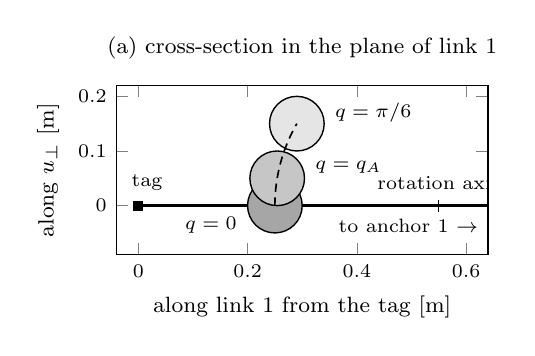
\begin{tikzpicture}\begin{axis}[width=6.3cm,height=5.0cm,axis equal image,xmin=-0.04,xmax=0.64,ymin=-0.09,ymax=0.22,xlabel={along link 1 from the tag [m]},ylabel={along $u_\perp$ [m]},title={(a) cross-section in the plane of link 1},title style={font=\footnotesize},label style={font=\footnotesize},tick label style={font=\scriptsize},xtick={0,0.2,0.4,0.6},ytick={0,0.1,0.2}]
\addplot[line width=1.0pt] coordinates {(0,0) (0.64,0)};
\node[font=\scriptsize,anchor=north east] at (axis cs:0.64,-0.006) {to anchor 1 $\rightarrow$};
\addplot[only marks,mark=square*,mark size=1.6pt] coordinates {(0,0)};
\node[font=\scriptsize,anchor=south west] at (axis cs:-0.03,0.010) {tag};
\addplot[only marks,mark=+,mark size=2.2pt] coordinates {(0.55,0)};
\node[font=\scriptsize,anchor=south] at (axis cs:0.55,0.012) {rotation axis};
\draw[fill=gray!70,line width=0.5pt] (axis cs:0.25000,0.00000) circle[radius=0.05];
\node[font=\scriptsize,anchor=east] at (axis cs:0.19800,-0.03500) {$q=0$};
\draw[fill=gray!45,line width=0.5pt] (axis cs:0.25420,0.05000) circle[radius=0.05];
\node[font=\scriptsize,anchor=west] at (axis cs:0.30620,0.07000) {$q=q_A$};
\draw[fill=gray!20,line width=0.5pt] (axis cs:0.29019,0.15000) circle[radius=0.05];
\node[font=\scriptsize,anchor=west] at (axis cs:0.34219,0.17000) {$q=\pi/6$};
\draw[densely dashed,line width=0.6pt] plot coordinates {(0.25000,0.00000) (0.25001,0.00262) (0.25005,0.00524) (0.25010,0.00785) (0.25018,0.01047) (0.25029,0.01309) (0.25041,0.01570) (0.25056,0.01831) (0.25073,0.02093) (0.25092,0.02354) (0.25114,0.02615) (0.25138,0.02875) (0.25164,0.03136) (0.25193,0.03396) (0.25224,0.03656) (0.25257,0.03916) (0.25292,0.04175) (0.25330,0.04434) (0.25369,0.04693) (0.25411,0.04951) (0.25456,0.05209) (0.25502,0.05467) (0.25551,0.05724) (0.25602,0.05981) (0.25656,0.06237) (0.25711,0.06493) (0.25769,0.06749) (0.25829,0.07003) (0.25891,0.07258) (0.25956,0.07511) (0.26022,0.07765) (0.26091,0.08017) (0.26162,0.08269) (0.26235,0.08520) (0.26311,0.08771) (0.26388,0.09021) (0.26468,0.09271) (0.26550,0.09519) (0.26634,0.09767) (0.26721,0.10014) (0.26809,0.10261) (0.26900,0.10506) (0.26993,0.10751) (0.27087,0.10995) (0.27184,0.11238) (0.27284,0.11481) (0.27385,0.11722) (0.27488,0.11962) (0.27594,0.12202) (0.27701,0.12441) (0.27811,0.12679) (0.27922,0.12915) (0.28036,0.13151) (0.28152,0.13386) (0.28270,0.13620) (0.28390,0.13852) (0.28512,0.14084) (0.28635,0.14315) (0.28761,0.14544) (0.28889,0.14773) (0.29019,0.15000)};
\end{axis}\end{tikzpicture}\hspace{2mm}\begin{tikzpicture}\begin{axis}[width=5.6cm,height=5.0cm,xmin=-0.06,xmax=0.10,ymin=0,ymax=1.08,xlabel={clearance $c$ [m]},ylabel={normalized weight},title={(b) calibration envelopes},title style={font=\footnotesize},label style={font=\footnotesize},tick label style={font=\scriptsize},scaled x ticks=false,xtick={-0.04,0,0.04,0.08},xticklabels={$-0.04$,$0$,$0.04$,$0.08$},legend style={font=\scriptsize,at={(0.97,0.03)},anchor=south east,draw=none,fill=none}]
\addplot[line width=1.0pt] table[x=c,y=u] {plot_env.dat};
\addlegendentry{$\psi^{+}$}
\addplot[line width=1.0pt,densely dashed] table[x=c,y=l] {plot_env.dat};
\addlegendentry{$\psi^{-}$}
\end{axis}\end{tikzpicture}\hspace{2mm}\begin{tikzpicture}\begin{axis}[width=5.6cm,height=5.0cm,xmin=0,xmax=0.5236,ymin=0.2,ymax=1.42,xlabel={$q$ [rad]},ylabel={index value},title={(c) indices and their bounds},title style={font=\footnotesize},label style={font=\footnotesize},tick label style={font=\scriptsize},xtick={0,0.1,0.2,0.3,0.4,0.5},legend style={font=\scriptsize,at={(0.98,0.03)},anchor=south east,draw=none,fill=white}]
\addplot[line width=0.5pt,gray] table[x=q,y=fpA] {plot_phi.dat};
\addlegendentry{$f^{+}$}
\addplot[line width=1.0pt] table[x=q,y=phip] {plot_phi.dat};
\addlegendentry{$\Phi^{+}$}
\addplot[line width=1.0pt,densely dashed] table[x=q,y=phim] {plot_phi.dat};
\addlegendentry{$\Phi^{-}$}
\addplot[line width=0.5pt,gray,densely dashed] table[x=q,y=fmA] {plot_phi.dat};
\addlegendentry{$f^{-}$}
\end{axis}\end{tikzpicture}
\end{document}
